\documentclass[conference]{IEEEtran}

\usepackage{cite}

\usepackage[cmex10]{amsmath}
\usepackage{amssymb}

\usepackage{algorithm}
%\usepackage{algorithmic}
\usepackage{algpseudocode}
\usepackage{indentfirst}
%\renewcommand{\algorithmicrequire}{ \textbf{Initialization:}}
%\renewcommand{\algorithmicensure}{ \textbf{Recurrence:}}

% Graph package
\ifx\pdfoutput\undefined
\usepackage{graphicx}
\else
\usepackage[pdftex]{graphicx}
\fi
\usepackage{epstopdf}

\usepackage{multirow}

\usepackage{courier}	%use courier font, activate using \texttt{}



% *** SUBFIGURE PACKAGES ***
\usepackage[tight,footnotesize]{subfigure}
% subfigure.sty was written by Steven Douglas Cochran. This package makes it
% easy to put subfigures in your figures. e.g., "Figure 1a and 1b". For IEEE
% work, it is a good idea to load it with the tight package option to reduce
% the amount of white space around the subfigures.


%\usepackage[caption=false]{caption}
%\usepackage[font=footnotesize]{subfig}
% subfig.sty, also written by Steven Douglas Cochran, is the modern
% replacement for subfigure.sty. However, subfig.sty requires and
% automatically loads Axel Sommerfeldt's caption.sty which will override
% IEEEtran.cls handling of captions and this will result in nonIEEE style
% figure/table captions. To prevent this problem, be sure and preload
% caption.sty with its "caption=false" package option. This is will preserve
% IEEEtran.cls handing of captions. Version 1.3 (2005/06/28) and later
% (recommended due to many improvements over 1.2) of subfig.sty supports
% the caption=false option directly:
\usepackage[caption=false,font=footnotesize]{subfig}








% correct bad hyphenation here
\hyphenation{op-tical net-works semi-conduc-tor}

\begin{document}

% can use linebreaks \\ within to get better formatting as desired
\title{Efficient FPGA Implementation of\\ Digit Parallel Online Arithmetic Operators}


% author names and affiliations
\author{Authors removed for blind review\\ \\ \\}
%\author{\IEEEauthorblockN{Kan Shi, David Boland, and George A. Constantinides}
%\IEEEauthorblockA{Department of Electrical and Electronic Engineering\\
%Imperial College London\\London, UK\\
%\{k.shi11, david.boland03,g.constantinides\}@imperial.ac.uk}
%}

\maketitle


\begin{abstract}
%\boldmath
Online arithmetic has been widely studied for ASIC implementation. Online components are designed to perform computations most significant digit first, resulting in the ability to chain arithmetic operators together for low latency. Recent research also shows that digit parallel online operators can fail more gracefully when operating beyond the deterministic clocking region, in comparison to operators with conventional arithmetic. Unfortunately, the utilization of online arithmetic operators in the past has required a large area overhead for FPGA implementation. In this paper, we propose novel approaches to implement the key primitives of online arithmetic, adders and multipliers, efficiently on modern Xilinx FPGAs with 6-input LUTs and carry resources. We demonstrate experimentally that in comparison to a direct implementation, the proposed architectures achieve over $67\%$ slice savings and over $1.2\times$ speed-ups for adders, and more than $3\times$ slice savings and $1.5\times$ speed-ups for multipliers. Furthermore in comparison to standard arithmetic primitives, the area overheads of online operators drop from $8.41\times$ to $1.88\times$ for adders, and $8.11\times$ to $0.54\times$ for multipliers using our approach.



\end{abstract}


% For peer review papers, you can put extra information on the cover
% page as needed:
% \ifCLASSOPTIONpeerreview
% \begin{center} \bfseries EDICS Category: 3-BBND \end{center}
% \fi
%
% For peerreview papers, this IEEEtran command inserts a page break and
% creates the second title. It will be ignored for other modes.
%\IEEEpeerreviewmaketitle



\section{Introduction}\label{Sec:Intro}
In the conventional form of computer arithmetic, the computation results are generated either from the least significant digit (LSD), e.g. addition and multiplication, or from the most significant digit (MSD), e.g. division and square root. This inconsistency in computing directions potentially results in large latency when propagating data between different operations. Online arithmetic was designed to solve this problem \cite{Ercegovac_OnlineOverview,Ercegovac_Book}. With online arithmetic, both inputs and outputs are processed in a MSD-first manner. This enables parallelism among multiple operations, and the overall computation latency can be significantly reduced. A brief overview of online arithmetic is given in Section~\ref{Sec:Background}.

Recent research has demonstrated another key advantage of online arithmetic: that it allows graceful degradation when operating beyond the deterministic clocking region, i.e. when overclocking \cite{SKDAC14_REVIEW}. This theme of research stems from the inspiration that for certain applications, releasing the absolute accuracy requirements could lead to significant performance improvements. However, traditional forms of computer arithmetic do not fail gracefully when timing violation happens, because timing errors tend to affect MSDs of the results. In comparison, online arithmetic is more ``overclocking friendly'', as timing errors only occur at LSDs of the results.

Despite its attractiveness, the use of online arithmetic on existing FPGAs is still limited due to a large area overhead. Given for standard arithmetic, it is difficult to efficiently map arithmetic circuits solely onto look-up-tables (LUTs), the fundamental building blocks of FPGAs. As a result, both main commercial FPGA vendors introduced dedicated carry logic into the logic block to reduce carry propagation delay~\cite{Virtex6}. Significant prior work explores methods that can effectively map circuits to the carry logic for performance improvements~\cite{FPL10_FPGA_CarryChain,Prefix_CarryChain}, or proposes alternative carry logic for FPGAs~\cite{FPGA_CarryChain_New1,FPGA_CarryChain_New2}. Hard DSP blocks are also included in modern architectures to improve the area and performance of multiplications and multiply accumulates~\cite{XilinxDSP}. However, most of these approaches are designed to accelerate computations with the conventional form of arithmetic.

For online arithmetic, two major research directions have been investigated. First, although there has been previous research into FPGA implementations of online arithmetic, this work only focused on online adders; a brief review of relevant works in this area is presented in Section~\ref{Sec:OA_FPGA}. Second, there are existing approaches to build general purpose online adders specifically for FPGAs with 4-input LUTs and with two LUTs within a slice or a logic element (LE), such as the Xilinx Spartan~3 series \cite{XilinxSpartan} and the Altera Cyclone III \cite{AlteraCyclone}. However, as will be discussed in Section~\ref{Sec:OA_FPGA}, these approaches cannot be directly applied on many modern FPGA with 6-input LUTs and four LUTs in a slice, such as the Xilinx Virtex series FPGAs and all Xilinx 7 series FPGAs~\cite{Virtex7}. Moreover, the move to the 6-LUT on the basic architecture opens new opportunities for efficient implementation.
%However, the implementations of other key arithmetic primitives, such as online multipliers, lack exploration.

In this paper, both issues will be addressed. In Section~\ref{Sec:OA_FPGA}, we propose a novel approach to map the digit parallel online adders onto FPGAs with 6-LUTs. The mapping is based on the fast carry logic, and the available resources within a slice can be fully utilized. In Section~\ref{Sec:OM_FPGA}, we optimize the online multiplication algorithm to yield an efficient FPGA implementation of a digit parallel online multiplier. The resource usage of both operators can be determined analytically. We demonstrate experimentally on Xilinx Virtex-6 FPGAs that the proposed designs achieve significant area reduction and performance gain over their original implementations. For online adders, our method achieves over $67\%$ slice savings and $1.2\times$ frequency speed-ups in comparison to a direct implementation. The area overhead drops from up to $8.41\times$ to $1.88\times$ using the proposed online adder in comparison to the standard ripple-carry adder. For online multipliers, the LUTs and slice utilization of the proposed new architecture drops over $2.4\times$ and $3.2\times$, with a frequency speed-up more than $1.5\times$ in comparison to a direct implementation. When compared to the multiplier with standard arithmetic, the direct implementation has an area overhead up to $8.11\times$. This value drops to $1.84\times$ when using the proposed online multiplier. In addition, using the proposed structure can even achieve area savings of up to $55\%$ for half precision results in comparison to the standard multiplier. 

In summary, the main contributions of this paper are efficient methods to map online adders and multipliers to modern FPGAs. 
% by fully utilizing the fast carry logic for .


%\begin{enumerate}
%    \item An efficient approach of mapping online adders onto modern FPGAs;
%    \item Area efficient implementation of digit parallel online multiplication algorithm on FPGAs;
%    \item Theoretical area models of the proposed architectures.
%\end{enumerate}


\section{Background: Online Arithmetic}\label{Sec:Background}
\subsection{Key Features of Online Arithmetic}

Online arithmetic has been widely used in numerous applications such as signal processing and control algorithms~\cite{Online_FPGADSP,Online_Control}. Online arithmetic was originally designed for digit-serial operation, as illustrated in Fig~\ref{Fig:OnlineDataFlow}. It can be seen that in order to generate the first output digit, $\delta$ digits of inputs are required, where $\delta$ is called the ``online delay''. $\delta$ is normally a small constant, which is independent of the precision. For ease of discussion, for the rest of this paper, the input data is assumed to be fixed point numbers in the range $(-1,1)$. Based on this premise, the online representation of $N$-digit operands and result at iteration $j$ are given by (\ref{Eq:Online_Operands}), where $j\in[-\delta,N-1]$ and $r$ denotes the radix \cite{Ercegovac_Book}.
%
\begin{figure}[tbp]
  \centering
  %\vspace{-2.5ex}
  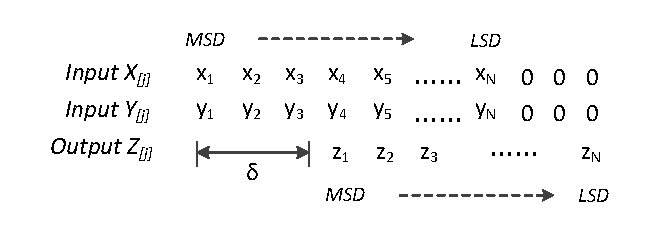
\includegraphics[width=.48\textwidth]{./Figures/OnlineArithmetic_DataFlow.pdf}
  \vspace{-4ex}
  \caption{Dataflow in digit-serial online arithmetic, in which both inputs and outputs are processed from the MSD to the LSD. $\delta$ denotes the online delay.}
  \vspace{-1ex}
  \label{Fig:OnlineDataFlow}
\end{figure}
%
\begin{eqnarray}\label{Eq:Online_Operands}
\footnotesize
  X_{[j]}=\sum_{i=1}^{j+\delta}x_ir^{-i},~Y_{[j]}=\sum_{i=1}^{j+\delta}y_ir^{-i},~Z_{[j]}=\sum_{i=1}^{j}z_ir^{-i}
\normalsize
\end{eqnarray}

MSD-first operation is possible only if a redundant number system is used. Normally there are two most commonly used redundant number representations: carry-save (CS) \cite{CSadder} and signed-digit (SD) \cite{RedundantNumber}. With SD representation, each digit is represented using a redundant digit set $\{-a, \cdots,-1,0, 1, \cdots, a\}$, where $a\in[r/2,r-1]$. In comparison, the standard non-redundant representation only uses a digit set $\{0,\cdots,r-1\}$. Thus a standard number corresponds to several possible redundant representations. For example, the binary number $0.011$ can be represented in SD form as $0.1\overline{1}1$, $0.10\overline{1}$ or $0.011$ among many other possible representations.

Due to the redundancy, the MSDs of the result can be calculated using partial information from both inputs. Then the value of the number can be revised using the subsequent digits, because each number has multiple representations.

\subsection{Binary Online Addition}
Adders serve as a critical building block for arithmetic operations. To perform digit-parallel online addition, a redundant adder can be used directly. The structure of an online adder where all signals represented with SD numbers of digit set $\{-1,0,1\}$ is shown in Fig.~\ref{Fig:Radix2SD_adder}. The module ``3:2'' denotes a 3:2 compressor, which takes 3 inputs and generates 2 outputs, and is logically equivalent to a full adder (FA). A major advantage of the redundant number system over the standard ripple-carry based arithmetic is that the propagation of carry is eliminated, resulting in a precision-independent computation time for addition. As labelled in Fig.~\ref{Fig:Radix2SD_adder}, ideally the computation delay of this adder is only 2 FA delays for any operand word-length, with the cost of one extra FA for each digit of operands. This makes the online adder suitable for building up more complex arithmetic operators such as multipliers to accelerate the sum of partial products \cite{RedundantMult_1987}.

\begin{figure}[tbp]
	\centering
	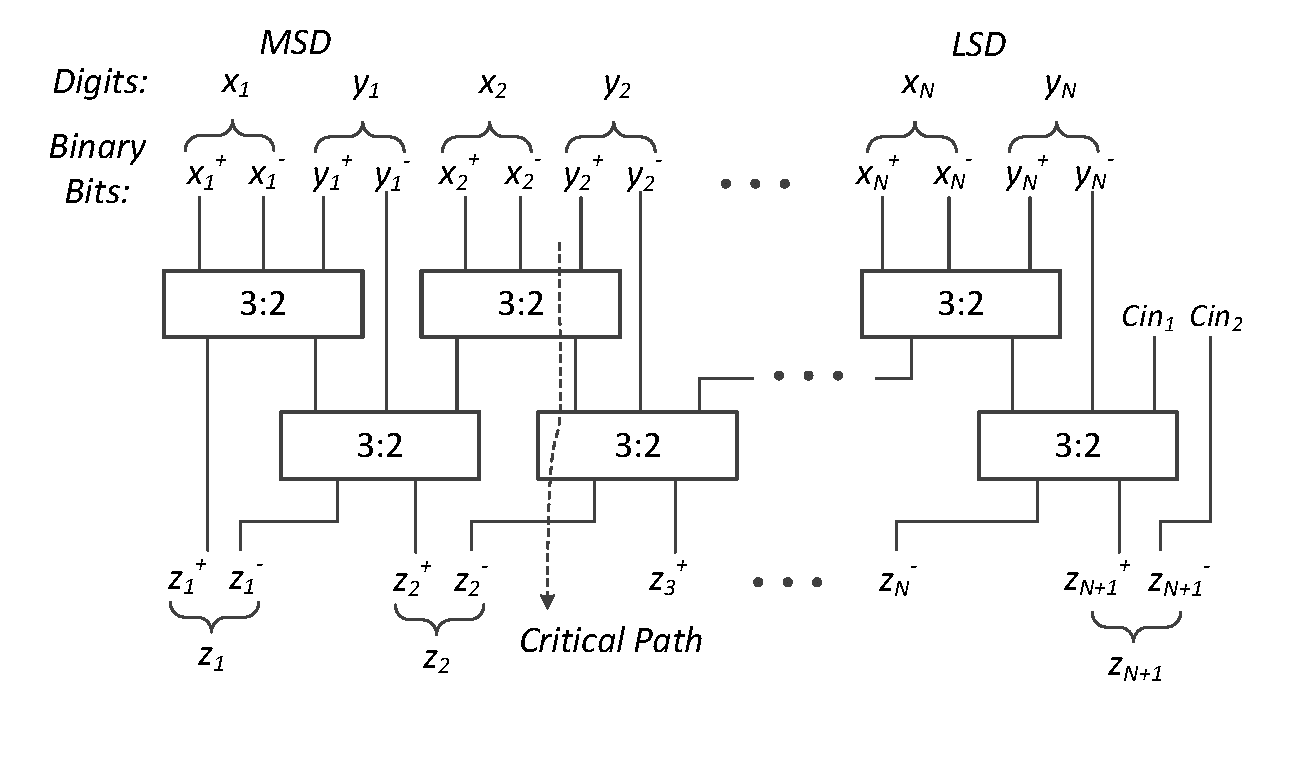
\includegraphics[width=.5\textwidth]{./Figures/SDAdder2.pdf}
    \vspace{-6ex}
	\caption{An $N$-digit binary digit-parallel online adder. Both inputs and outputs are represented using SD representation. ``3:2'' denotes a 3:2 compressor.}
    %\vspace{2ex}
	\label{Fig:Radix2SD_adder}
\end{figure}

%In Section~\ref{Sec:OA_FPGA}, we will present a novel method of mapping the digit parallel online adder efficiently on FPGAs using the built-in carry resources.

\subsection{Binary Online Multiplication}
Multiplication is another key arithmetic operator. Typically, online multiplication is performed in a recursive digit serial manner, as illustrated in Algorithm~\ref{Algorithm:OnlineMult} \cite{Ercegovac_OnlineMult} where both inputs and outputs are $N$-digit numbers as given in~(\ref{Eq:Online_Operands}). For a given iteration $j$, the product digit $z_j$ is generated MSD-first through a selection function $sel()$. For any radix $r$ and chosen digit set, there exits an appropriate selection method and a value of $\delta$ which ensure convergence. As the binary radix is used most commonly in computer arithmetic, we keep $r=2$ throughout this paper with the corresponding redundant digit set $\{\overline{1},0,1\}$. In this case $sel()$ is given by (\ref{Eq:SelFunc_OM}), and the selection is based on two integer digits and one fractional digit of $W_{[j]}$ \cite{Ercegovac_OnlineMult}.
%
\begin{algorithm}[tbp]
  \caption{Online Multiplication}  \label{Algorithm:OnlineMult}
  \begin{algorithmic}[1]
   \State \textbf{Initialization:}~$X_{[-\delta]}=Y_{[-\delta]}=P_{[-\delta]}=0$\vspace{.5ex}
    \For{$j=-\delta,~-\delta+1,~\cdots,~2N-1$}\vspace{.5ex}
        \State $H_{[j]} \leftarrow r^{-\delta}\left(x_{j+\delta+1}\cdot Y_{[j+1]}+y_{j+\delta+1}\cdot X_{[j]}\right)$\vspace{.5ex}
        \State $W_{[j]} \leftarrow P_{[j]} + H_{[j]}$\vspace{.5ex}
        \State $z_{j}~ \leftarrow sel(W_{[j]})$\vspace{.5ex}
        \State $P_{[j+1]} \leftarrow r\left(W_{[j]}-Z_{[j]}\right)$\vspace{.5ex}
    \EndFor
  \end{algorithmic}
\end{algorithm}

\begin{eqnarray}\label{Eq:SelFunc_OM}
%\small
  sel(W_{[j]})=\begin{cases}
    1 & \text{ if } W_{[j]} \geqslant \frac{1}{2} \\
    0 & \text{ if } -\frac{1}{2}\leqslant W_{[j]}<\frac{1}{2} \\
    \overline{1} & \text{ if } W_{[j]}<-\frac{1}{2}
  \end{cases}
%\normalsize
\end{eqnarray}

It is worth noting that the precision of the product $Z$ can be determined by directly truncating from the LSDs, since there is no carry propagation from the LSD to the MSD. This is useful especially when the multiplication product is used by successive computations, where often only the first $N$ digits of the results are used. In comparison, the product is generated starting from the LSD with conventional arithmetic. Hence the successive operations cannot commence until the result with full-precision is generated. This feature of online arithmetic has inspired research about dynamically control of computation precision in numerous applications~\cite{Online_Truncation}.

%Since there is no carry chain propagating from the LSD to the MSD, the precision of the results can be selected by directly truncating from the LSDs.

In Section~\ref{Sec:OM_FPGA}, we will first describe an optimized online multiplication algorithm and its FPGA implementation, which are designed specifically targeting digit parallel operations. Then we provide a modified structure which only generates the most significant half of the product in order to achieve extra area savings.

%\subsection{FPGA Architecture}


\section{Digit Parallel Online Adder for FPGAs}\label{Sec:OA_FPGA}
\subsection{Related Works}
There have been previous works about FPGA implementation of digit parallel online adders. From the literature, the existing approaches can be classified into three types:

\begin{enumerate}
    \item efficient mapping of the digit-parallel online adder onto sophisticated FPGAs resources \cite{FPT09RA,ASAP09RA};
    \item multiple operand addition by designing compressor trees based on bit counters \cite{TC13RA,CSMult_CounterArray};
    \item modifying existing FPGA architecture for more efficient digit-parallel online addition \cite{DAC07_CounterTree} and for specific applications \cite{FPL09_onlineCCM}.
\end{enumerate}

Type 2 examines the use of counters to sum $k$ $N$-digit numbers where $k>2$. Instead, we focus on two-operand online addition that performs $Z=X+Y$, as shown in Fig.~\ref{Fig:Radix2SD_adder}. In comparison to type 3, this paper attempts to obtain the best performance from mainstream FPGAs instead of suggesting ways to modify the FPGA fabric.

Specifically in type 1, both works took advantage of the built-in carry resources in FPGAs. Conventionally the ASIC implementation of online adders is based on 4:2 compressors, as outlined in Fig.~\ref{Fig:PreviousWork} within the gray background. However, directly applying this approach in the FPGAs could be less efficient. This is because there is no carry propagation between the two FAs within a 4:2 compressor, and the net delay between them can be large. Instead, Kamp et al \cite{FPT09RA} and Hormigo et al \cite{ASAP09RA} described very similar mapping techniques for online adders with SD representations and CS representations, respectively. They share the common idea of building the online adder based on the logic block (\texttt{LB}) as highlighted within the dotted circle in Fig.~\ref{Fig:PreviousWork}. In this case, the fast-carry logic in the FPGA can be employed, and the delay between the two 3:2 compressors can be greatly reduced.

\begin{figure}[tbp]
	\centering
	\includegraphics[width=.5\textwidth]{./Figures/SDAdder_42comp_Spartan2.pdf}
	\caption{Map the online adder onto Spartan FPGAs using the fast-carry resources. The gray background highlights the 4:2 compressor. Dotted circle indicates the logic block (LB) which can be mapped to the FPGA using the carry resources.}
	\label{Fig:PreviousWork}
\end{figure}

However, we notice the major limitations of both approaches that they only target FPGAs with 4-input LUTs (4-LUT) and two LUTs within a logic slice, such as the Xilinx Spartan series and the Altera Cyclone series. This is naturally reasonable because one \texttt{LB} can be mapped to a single slice. Nevertheless, for FPGAs with 6-input LUTs (6-LUT) and four LUTs in a slice, such as the Xilinx Virtex series and all Xilinx 7 series FPGAs, directly applying these approaches will result in either resource waste or wrong results. For instance, if two \texttt{LB}s are mapped to a slice with four LUTs as seen in Fig.~\ref{Fig:PreWorkVirtex6}, the outputs of \texttt{LB1} should not be used because the its carry input cannot be explicitly initialized. Due to the same reason, the output of \texttt{XORCY2} should not be used.

\begin{figure}[tbp]
	\centering
	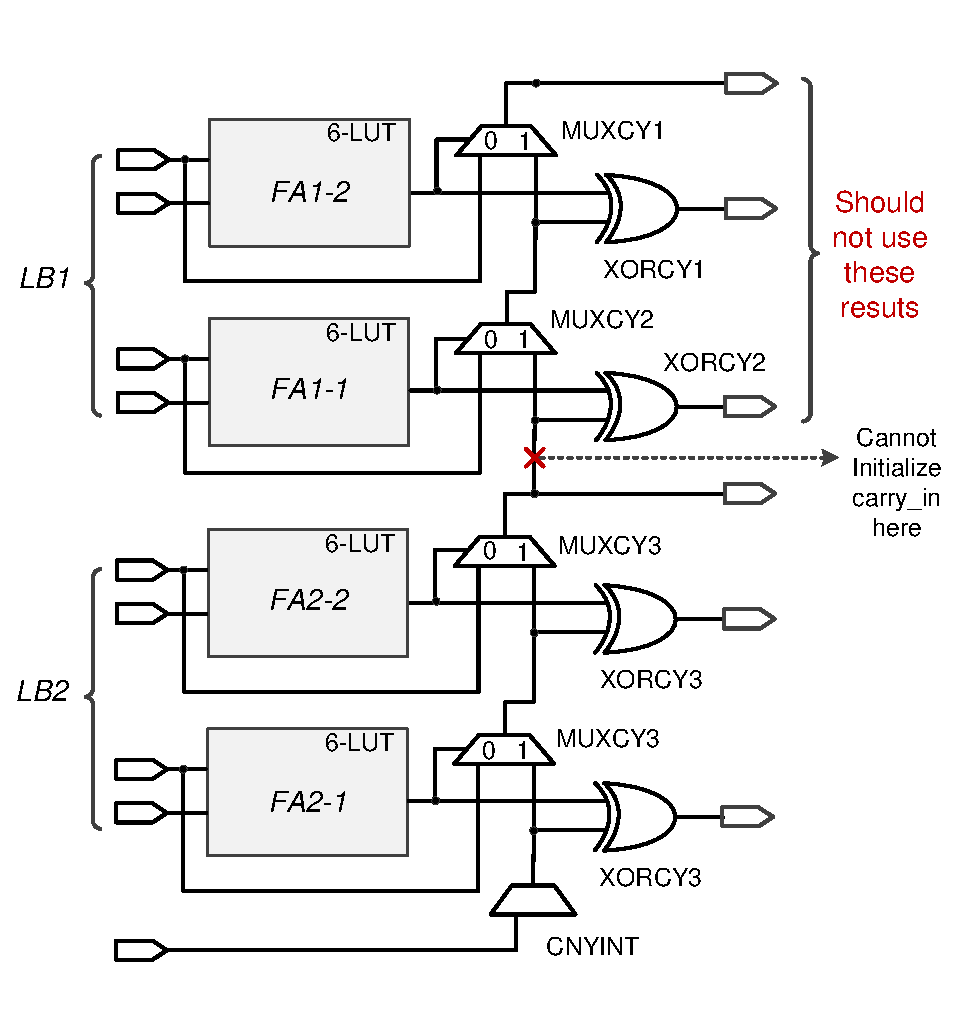
\includegraphics[width=.45\textwidth]{./Figures/SDadder_FastCarry_PreviousWork2.pdf}
	\caption{An example illustrating that direct applying approaches in \cite{FPT09RA} on a Virtex-6 FPGA will results in faulty outputs, because the carry input of \texttt{LB1} cannot be explicitly initialized.}
	\label{Fig:PreWorkVirtex6}
    %\vspace{-2ex}
\end{figure}

\subsection{Proposed Mapping Method}
To tackle this problem, we first present an alternative structure of the online adder to enable an efficient FPGA mapping. The structure of a 4-digit online adder is given as an example in Fig.~\ref{Fig:ModifiedOA}. In this equivalent structure, the first FA in each 4:2 compressor is split into two parts, which only generate carry and sum respectively. In this case they can be mapped individually on two LUTs. The second FA, which generates the outputs, is unchanged and can be implemented using the fast carry logic.


%propose an alternative mapping method that targets on the slice containing 4 LUTs such as the Xilinx Virtex series and all Xilinx 7 series FPGAs.

\begin{figure*}[tbp]
	\centering
	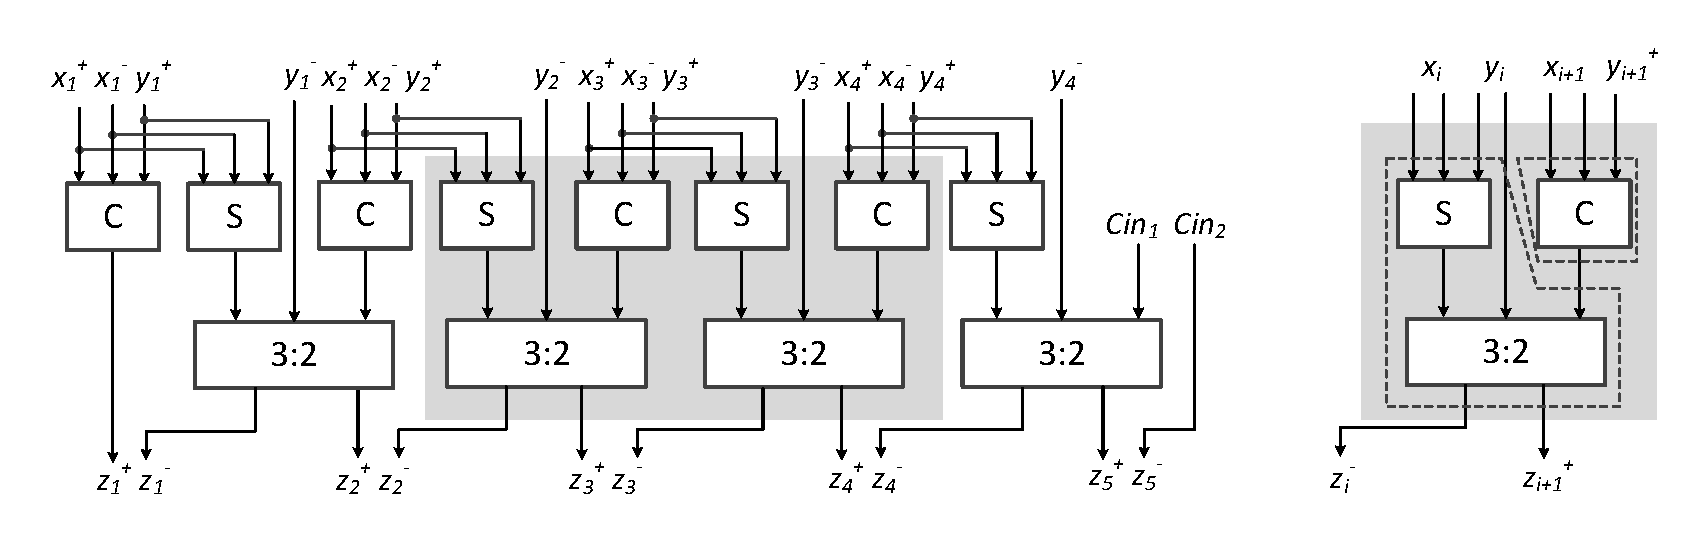
\includegraphics[width=.85\textwidth]{./Figures/SDadder_FPGA_New_4digit2.pdf}
	\caption{Alternative structure of online adder. Left: an example of 4-digit online adder. The shaded part refers to the 2 logic blocks (LBs) that can be mapped onto 1 slice. Right: one LB. The dotted boxes outline the logic that can be mapped onto each LUT and the corresponding fast carry logic.}
	\vspace{-1ex}	
	\label{Fig:ModifiedOA}
\end{figure*}

The detailed slice mapping of the two \texttt{LB}s and the logic in each LUT are shown in Fig.~\ref{Fig:SliceNew}. The I/O signals are identical to the previous example in Fig.~\ref{Fig:ModifiedOA}. The 6-LUT can be configured with two different output ports \texttt{O6} and \texttt{O5}. For \texttt{LB1}, the carry input can be initialized by setting the \texttt{O6} of LUT2 to 0. In this case, the output of \texttt{MUXCY2} is always \texttt{O5} of LUT2, and the carry from \texttt{LB2} will not affect the result of \texttt{LB1}. The logic to generate the MSD and the LSD can be combined into one slice as observed from Fig.~\ref{Fig:ModifiedOA}. Therefore using this mapping method the resources within one slice can be fully utilized, leading to a significant area reduction.

\begin{figure}[tbp]
	\centering
	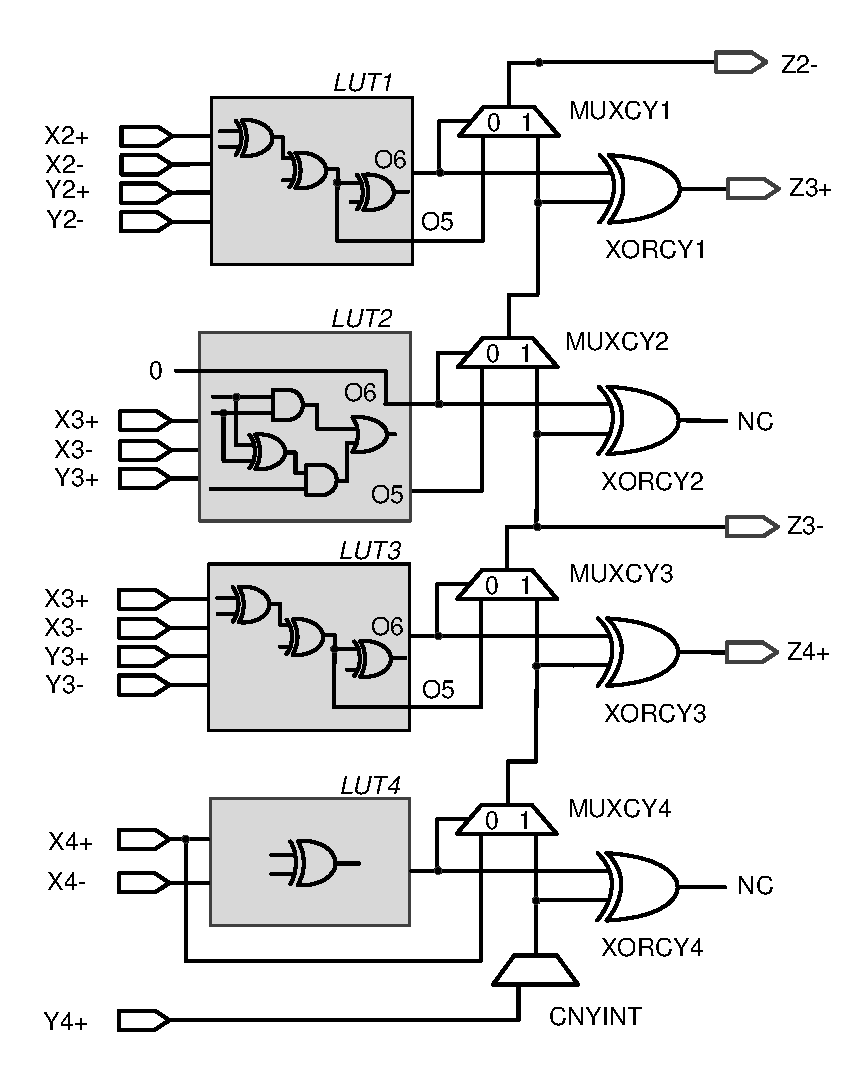
\includegraphics[width=.5\textwidth]{./Figures/SDadder_FastCarry_New2.pdf}
	\caption{Implementation of 2 logic blocks (LBs) in 1 FPGA slice which contains four 6-LUTs. NC stands for ``Not Care''.}
	%\vspace{-1ex}	
	\label{Fig:SliceNew}
\end{figure}

In this mapping approach, the area figures of the online adder in terms of the number of LUTs and slices with respect to the operand word-lengths ($N$) are given in (\ref{Eq:OAareaLUT}) and (\ref{Eq:OAareaSlice}), respectively.
\begin{eqnarray}\label{Eq:OAareaLUT}
	OA\_LUT = 2N
\end{eqnarray}
%
\begin{eqnarray}\label{Eq:OAareaSlice}
	OA\_slice = 1+\left\lceil\frac{N-2}{2}\right\rceil
\end{eqnarray}

\subsection{Performance Analysis}\label{subsec:OA_Performance}
In our experiments, we compare the proposed online adder (\texttt{OA\_new}) against the original design which is implemented using functional descriptions in Verilog based on 4:2 compressors (\texttt{OA\_behv}).  In addition, we also include ripple carry adder (\texttt{RCA}) which uses conventional arithmetic, into the comparisons. While in our experiments all designs are targeting on Xilinx Virtex-6 FPGA with speed grade -1, our methods can also be applied on other FPGAs with same slice architecture such as the Xilinx 7 series FPGAs. Notice that in order to utilize the carry resources and to avoid logic optimizations by the synthesis tool, the Xilinx primitive component ``\texttt{Carry4}" is used to create \texttt{OA\_new}.

\begin{figure}[tbp]
	\centering
	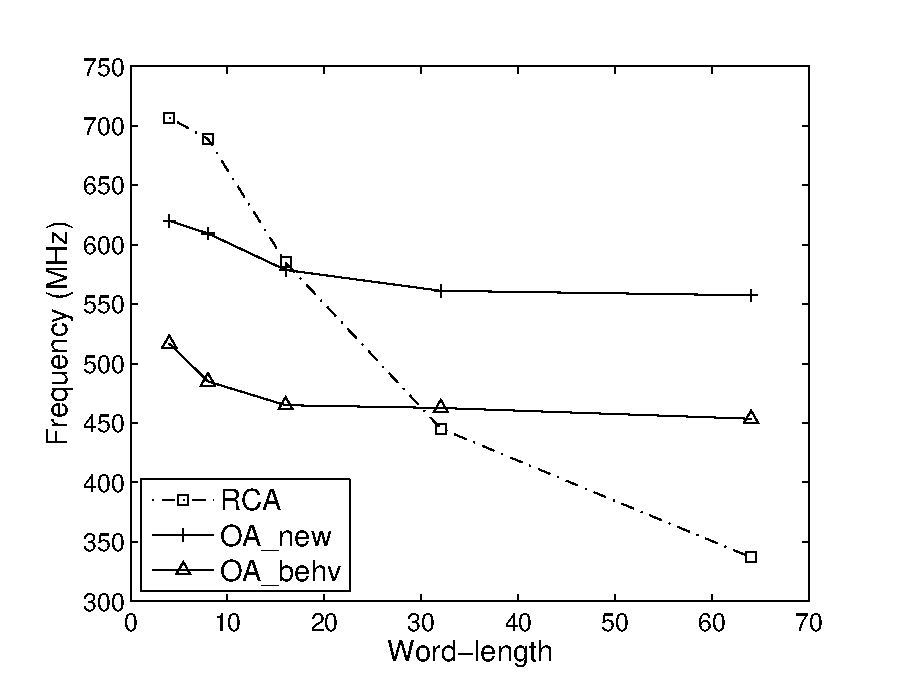
\includegraphics[width=.45\textwidth]{./Figures/Exp/Adder_Freq.eps}
	\caption{Rated frequencies of the RCA and the online adder with different implementation methods. The results are obtained from post place and route timing reports in ISE 14.1.}
	\label{Fig:AdderFreq}
	\vspace{-1ex}
\end{figure}


We record the rated frequencies of all designs when varying the operand word-lengths. The results are shown in Fig.~\ref{Fig:AdderFreq}. The frequency values are obtained through Xilinx Timing Analyzer after placing and routing the designs in ISE 14.1. It can be seen that both designs with online arithmetic achieves relatively stable operating frequencies across a variety of operand word-lengths. This is as expected, because the critical path delay in the online adder is theoretically a fixed value independent of the operand precision. In comparison, the rated frequency of the \texttt{RCA} drops dramatically for larger word-lengths. It follows that both online adders outperform \texttt{RCA} for large word-lengths. Specifically, the frequency of \texttt{OA\_behv} is faster than \texttt{RCA} when $N\geqslant30$. In comparison, the proposed online adder is more efficient in performance, as it outperforms \texttt{RCA} for $N>16$. Furthermore, the speed-ups of \texttt{OA\_new} over \texttt{OA\_behv} are from $1.20\times$ to $1.26\times$.



We also compare the resource usage of all three adder designs with respect to a variety of operand word-lengths. The results are presented in Fig~\ref{Fig:AdderArea}. We can see that in comparison to the original \texttt{OA\_behv}, our implementation \texttt{OA\_new} achieves significant area savings: $25\%\sim 33\%$ in LUTs and $67\%\sim77\%$ in slices. This is because the dedicated FPGA resources are fully utilized. However, our design still costs more area than an \texttt{RCA}, with an area overhead of $80\%\sim98\%$ in terms of LUTs, and up to $88\%$ in terms of slices. This is because for a single adder, the area overhead brought by the redundant number representations cannot be removed.
%However research has shown that this overhead can be reduced for multiple-operand adders or adder trees [xxx].

\begin{figure}[tbp]
  %\vspace{-2.5ex}
  \centering
  \subfigure[Usage of LUTs]{
  \begin{minipage}{0.45\textwidth}
    %\centering
    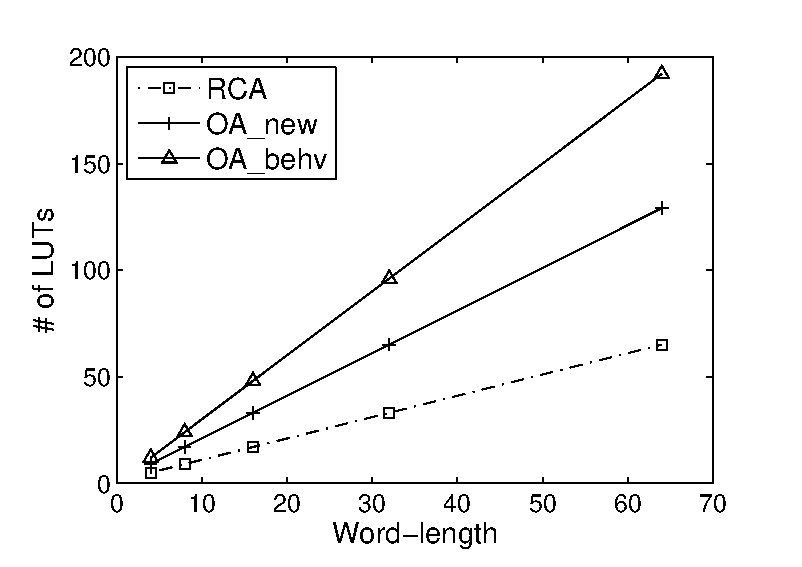
\includegraphics[width=.95\textwidth]{./Figures/Exp/Adder_LUTs3.eps}
    \vspace{1ex}
  \end{minipage}%
  }
  \subfigure[Usage of slices]{
  \begin{minipage}{0.45\textwidth}
    %\centering
    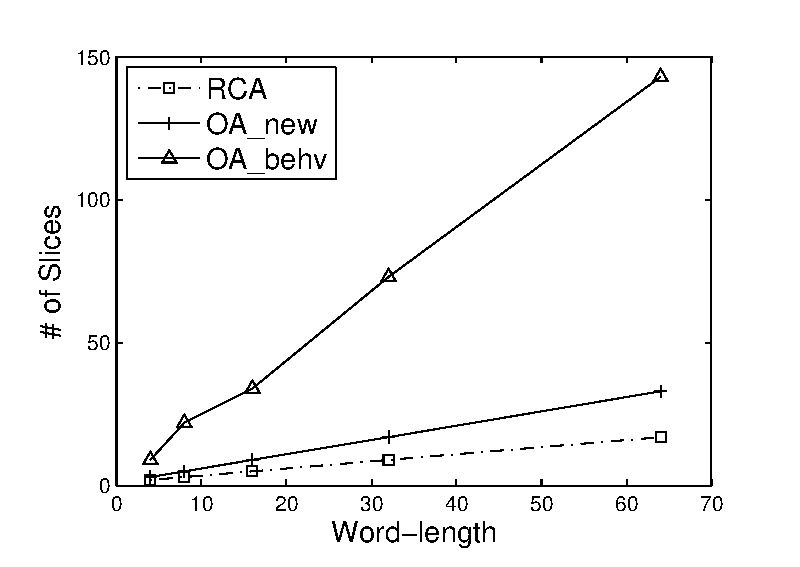
\includegraphics[width=.95\textwidth]{./Figures/Exp/Adder_Slices3.eps}
    \vspace{1ex}
  \end{minipage}
  }
  %\vspace{-3ex}
  \caption{Area comparisons of different binary adder implementations with respect to a variety of operand word-lengths.}
  \label{Fig:AdderArea}
  \vspace{-2ex}
\end{figure}






\section{Digit Parallel Online Multiplier on FPGAs}\label{Sec:OM_FPGA}
\subsection{Algorithm of Digit Parallel Online Multiplication}
Algorithm \ref{Algorithm:OnlineMult} as described in Section~\ref{Sec:Background} can be synthesized into a unrolled digit parallel structure. A recent study has shown that the digit-parallel online multiplier (\texttt{OM}) is also more tolerant to timing violations in comparison to the conventional arithmetic, because timing errors initially affect the LSDs and this will lead to smaller error magnitude~\cite{SKDAC14_REVIEW}. %This implementation method is straightforward and can be directly utilized to design other digit parallel online operators.

However, significant area overhead is required in order to implement this type of \texttt{OM}, due to three main reasons. First, in comparison to the conventional multiplier, more iteration stages are needed. For instance in an $N$-digit \texttt{OM}, $(2N+\delta)$ iterations are required to generate $2N$ digits outputs, or $(N+\delta)$ iterations are required to generate the most significant $N$ digits. Second, the logic of each stage is complex as it involves operations such as online addition, digit-vector multiplication (to generate $x_{j+\delta+1}\cdot Y_{[j+1]}$ and $y_{j+\delta+1}\cdot X_{[j]}$ in Algorithm~\ref{Algorithm:OnlineMult}), shifting and other combinational logic blocks such as the selection function. Also, the word-length of signals $H_{[j]}$, $W_{[j]}$ and $P_{[j]}$ is $(N+2+\delta)$, because the selection function needs two integer digits and one fractional digit to generate $z_j$, as described in Section~\ref{Sec:Background}. Third, this \texttt{OM} architecture is not optimized specifically for FPGA technology.
%In comparison, an $N$-digit array multiplier, there are only $(N-1)$ rows, each of which is basically an $N$-digit ripple-carry adder.

We address the first two design issues by providing an alternative online multiplication algorithm. Instead of simply implementing the unrolled version of Algorithm \ref{Algorithm:OnlineMult}, it can be optimized specifically for digit parallel operations. The online delay $\delta$ is employed in Algorithm~\ref{Algorithm:OnlineMult} because the input data is available in a digit serial fashion. Hence $\delta$ is used to accumulate enough input digits to generate the MSD of the result. However if all digits of the inputs are available simultaneously, then the delay $\delta$ is no longer necessary. For the same reason, $H[j]$, which takes one digit of each input per stage as shown in the original algorithm, can be optimized to take one partial product $Xy_j$ or $Yx_j$ per stage. To summarize, the modified algorithm for digit parallel online multiplication is described in Algorithm~\ref{Algorithm:OM_DigitParallel}, where $N$ denotes the operand word-length, function $frac(W_{[N]})$ refers to select the fractional digits of $W_{[N]}$, and the selection function $sel()$ is given previously in (\ref{Eq:SelFunc_OM}).

\begin{algorithm}[tbp]
  \caption{Digit Parallel Online Multiplication}\label{Algorithm:OM_DigitParallel}
  \begin{algorithmic}[1]
    \State \textbf{Initialization:} $P_{[0]}=0$						\vspace{.5ex}
    \For{$j=1,~2,~\cdots,~N$}										\vspace{.5ex}
    	\State $Xy_j \leftarrow X \cdot y_j$						\vspace{.5ex}
    	\State $W_{[j]}    \leftarrow  P_{[j-1]} + Xy_j$			\vspace{.5ex}
     	\State $z_{j}  ~~      \leftarrow  sel(W_{[j]})$			\vspace{.5ex}
	 	\State $P_{[j+1]}  \leftarrow  r\left(W_{[j]}-Z_{[j]}\right)$	\vspace{.5ex}
    \EndFor															\vspace{.5ex}
    \State $Z_{[N+1:2N]} \leftarrow frac(W_{[N]})$
  \end{algorithmic}
\end{algorithm}

In comparison to Algorithm~\ref{Algorithm:OnlineMult}, the maximum number of stages required to generate results with full precision drops by a factor of 2 using the proposed new algorithm. In each stage, the word-length of all signals also reduces from $(N+2+\delta)$ to $(N+2)$, as $\delta$ is not necessary for digit parallel operations. In addition, the $frac()$ function can be implemented only based on wire connections without using logic resources.

\subsection{FPGA Implementation}
We now present an area efficient implementation of Algorithm~\ref{Algorithm:OM_DigitParallel} on FPGAs. The general structure of a 4-digit \texttt{OM} using the proposed algorithm is shown in Fig.~\ref{Fig:PMStructure}(a), and the structure of a single stage $j$ is shown in Fig.~\ref{Fig:PMStructure}(b) with the word-lengths of all signals labelled. Area optimizations can be performed on all modules. It can be seen that in each stage, an $(N+2)$ digit online adder is used to derive $W_{[j]}$. Our proposed online adder architecture can be employed. The selection logic takes 3 input digits (6 bits) and generates 1 output digit (2 bits). Hence it can be implemented using two 6-LUTs for each output bit. Similarly the generation of $P_{[j]}$ can also be implemented using one 6-LUT, since only the integer digits of $W_{[j]}$ need to be modified due to the selection of $Z_{[j]}$. In addition, the structure of Stage 1 in Fig~\ref{Fig:PMStructure}(a) can be further optimized by removing the online adder, because $P_{[0]}=0$.
%
\begin{figure}[tbp]
	\centering
	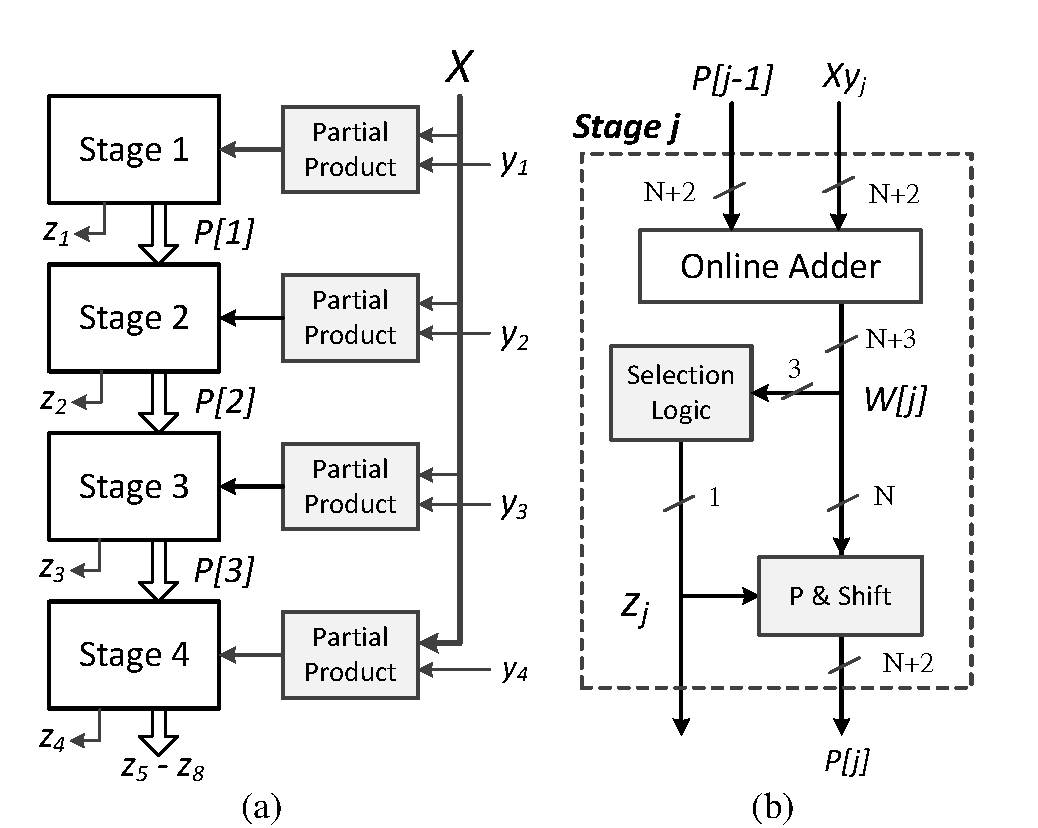
\includegraphics[width=.5\textwidth]{./Figures/ParallelMult_Structure.pdf}
	\caption{(a) Structure of a 4-digit online multiplier using the proposed algorithm. (b) Structure of one stage. The word-length of all signals are labelled in terms of the number of digits. $N$ denotes the word-length of the input signals.}
	\label{Fig:PMStructure}
	\vspace{-1ex}
\end{figure}

The blocks that generate partial products $Xy_j$ can be incorporated into the online adder for further area reduction. In the online adder structure as presented in Fig.~\ref{Fig:SliceNew}, we notice that only four inputs per LUT are used. This leaves at least two available inputs per LUT. Originally in order to generate one digit partial product, one digit of inputs $X$ and $Y$ are required respectively, as indicated in Fig.~\ref{Fig:PartialProduct}. Instead of using extra logic to generate $Xy_j$, it can be merged into the corresponding LUTs in the online adder by fully utilizing all six LUT inputs. Notice that this approach is only available for FPGAs with 6-LUTs.
%
\begin{figure}[tbp]
	\centering
	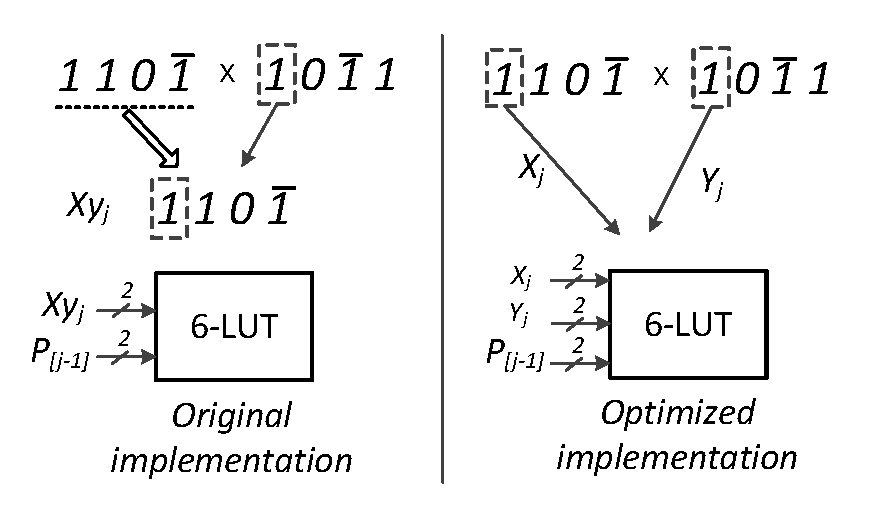
\includegraphics[width=.4\textwidth]{./Figures/PartialProduct.pdf}
	\vspace{-1ex}
	\caption{Left: Direct implementation with extra logic to generate partial products. Right: Combining the logic blocks that generate partial products into the Online Adder by fully utilizing all the inputs of the 6-LUTs. In this case, further area reduction can be achieved.}
	\label{Fig:PartialProduct}
	\vspace{-1ex}
\end{figure}

The resource usage of the proposed \texttt{OM} can be calculated as follows. In an $N$-digit \texttt{OM}, in total $(N-1)$ online adders are needed. According to Algorithm~\ref{Algorithm:OM_DigitParallel}, the word-length of each online adder is $(N+2)$-digit (two integer digits and $N$ fractional digits). Therefore based on (\ref{Eq:OAareaLUT}) and (\ref{Eq:OAareaSlice}), the number of LUTs and the number of slices used by the \texttt{OM} is given in (\ref{Eq:OMareaLUT}) and (\ref{Eq:OMareaSlice}), respectively. Note that $L_{S1}$ and $S_{S1}$ denote the number of LUTs and slices used by the first stage, which is built without online adders.

\begin{eqnarray}\label{Eq:OMareaLUT}
	OM\_{LUT} = 2(N+2)(N-1) + {L}_{S1}
\end{eqnarray}
%
\begin{eqnarray}\label{Eq:OMareaSlice}
	OM\_{slice} = \left(1+\left\lceil{\frac{N}{2}}\right\rceil\right)(N-1)+S_{S1}
\end{eqnarray}

\subsection{Structure Optimization for Half Precision Results}
As discussed before, normally the multiplier is connected with other arithmetic operators in real applications. If the outputs of a multiplier is utilized for subsequent operations, and a consistent word-length is used throughout the system, then only the most significant half of the product is required. In a conventional multiplier with standard binary arithmetic, this is achieved by either truncating or rounding the least significant half of the products. However, both the computation time and the structure remains unchanged, because the results are generated from LSDs.

\begin{figure}[tbp]
	\centering
	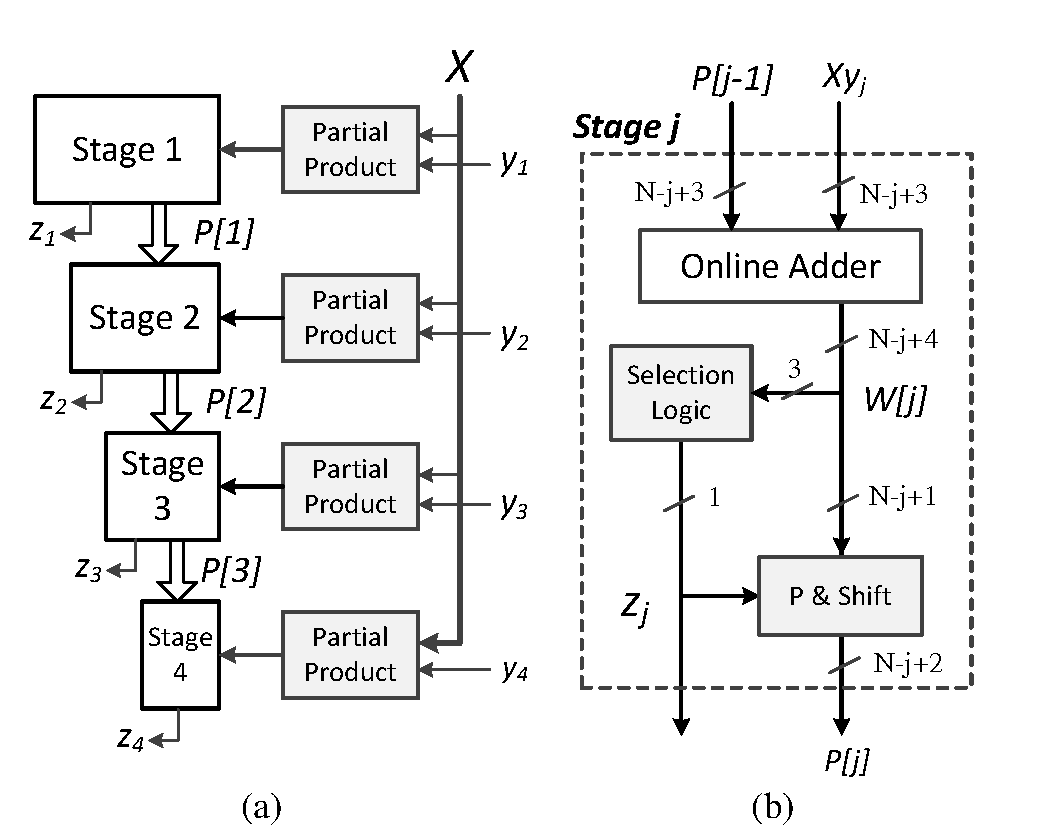
\includegraphics[width=.5\textwidth]{./Figures/ParallelMult_MSDhalf.pdf}
	\caption{(a) Modified structure of a 4-digit online multiplier which only generates the most significant 4-digit result. (b) Structure diagram of stage $j$, with the word-lengths of all internal signals labelled.}
	\label{Fig:PMStructure_MSDhalf}
	%\vspace{-2ex}
\end{figure}

In comparison, the \texttt{OM} offers the flexibility to simplify the structure corresponding to the required precision. This is possible because in an \texttt{OM}, the product digits are generated initially from the MSD, and there is no carry propagation from the LSD to the MSD with the employment of the redundant number system. This will potentially lead to a more area efficient design. For example, the modified structure diagram of a 4-digit \texttt{OM} is illustrated in Fig.~\ref{Fig:PMStructure_MSDhalf}(a). The word-length of signals within each stage can be correspondingly reduced, as shown in Fig.~\ref{Fig:PMStructure_MSDhalf}(b). It can be seen that instead of keeping identical word-length throughout the stages (in Fig.~\ref{Fig:PMStructure}), in the modified structure the signal word-lengths depend on the stage number $j$ and fewer bits of signals are needed for LSD stages.



\subsection{Performance Analysis}
Similar to the experiments as described in Section~\ref{subsec:OA_Performance}, we compare the direct RTL online multiplier (\texttt{OM\_behv}) against the proposed two types of multiplier, which are implemented to generate products with full precision (\texttt{OM\_full}) and half precision (\texttt{OM\_half}), respectively. In addition, we also compare the \texttt{OM} with the conventional binary arithmetic multiplier. The conventional multiplier is created using the Xilinx Core Generator with speed optimization~\cite{XilinxMult}, and it is implemented based on LUTs without DSPs for a fairer comparison.

The comparison of area in terms of the cost of LUTs and the cost of slices with respect to different operand word-lengths are illustrated in Fig.~\ref{Fig:OMArea}. The results are obtained from ISE 14.1 after mapping the design to the Virtex-6 FPGA. In comparison to \texttt{OM\_behv}, significant area savings have been obtained by the optimized design \texttt{OM\_full}. Specifically, the LUTs and slice utilization drops $2.44\times\sim3.34\times$ and $3.19\times\sim5.45\times$, respectively.

In comparison to the \texttt{CoreGen} multiplier, the area overhead of online multipliers drops significantly when transferring to the proposed new structure. In order to generate full precision product, the area overheads of \texttt{OM\_behv} against \texttt{CoreGen} are $3.94\times\sim5.82\times$ for LUTs, and $3.58\times\sim8.11\times$ for slices, respectively. Using the proposed structure \texttt{OM\_full} the area overheads drop to $1.48\times\sim1.83\times$ for LUTs and up to $1.84\times$ for slices. Furthermore, if only half precision result is required, \texttt{OM\_half} is more area efficient for all operand word-lengths when compared against the \texttt{CoreGen} multiplier. The area saving varies from $40\%$ to $55\%$ for LUTs, and $46\%$ to $55\%$ for slices.

\begin{figure}[tbp]
  %\vspace{-2.5ex}
  \centering
  \subfigure[Usage of LUTs]{
  \begin{minipage}{0.47\textwidth}
    %\centering
    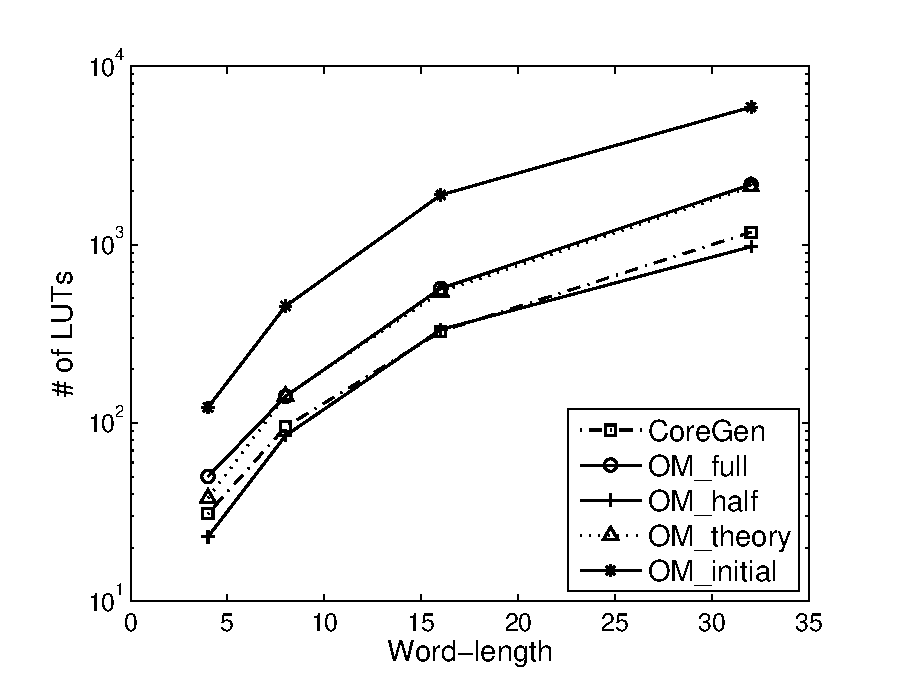
\includegraphics[width=.95\textwidth]{./Figures/Exp/OM_LUTslog.eps}
    \vspace{1ex}
  \end{minipage}%
  }
  \subfigure[Usage of slices]{
  \begin{minipage}{0.47\textwidth}
    %\centering
    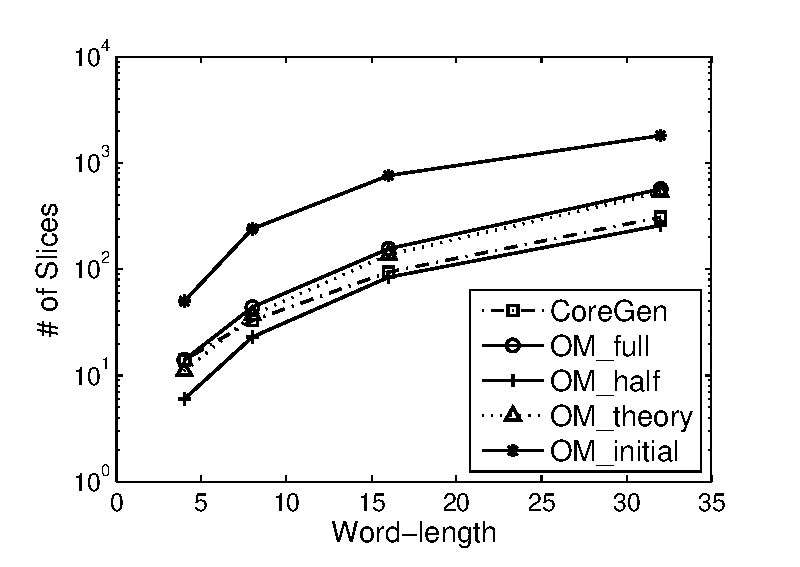
\includegraphics[width=.95\textwidth]{./Figures/Exp/OM_Slicelog.eps}
    \vspace{1ex}
  \end{minipage}
  }
  %\vspace{-3ex}
  \caption{Area comparisons of different types of binary multipliers.}
  \label{Fig:OMArea}
  %\vspace{-2ex}
\end{figure}

We also check the rated frequencies of all multipliers for a variety of operand word-lengths. The frequency values are plotted in Fig.~\ref{Fig:OM_Freq}, which are still obtained from the post place and route timing reports. In Fig.~\ref{Fig:OM_Freq} we see that in comparison to \texttt{OM\_behv}, our proposed architectures achieve frequency speed-ups varying from $1.49\times$ to $1.98\times$.

Notice that there is an increasing gap between the proposed online multipliers and the \texttt{CoreGen} multiplier, especially for large operand word-lengths. This is because in the online multiplier, although the carry resources in the FPGA are efficiently used for area reduction, each 4-digit carry logic within a slice is divided into two parts, as shown previously in Section~\ref{Sec:OA_FPGA}. Therefore the critical path delay of an \texttt{OM} is determined by both the carry logic delays, and the net delay among different stages, which is hyperbole for large operand word-lengths. This also explains the fact that \texttt{OM\_full} and \texttt{OM\_half} run at similar frequencies, as the critical path of both designs are identical in theory.

\begin{figure}[tbp]
	\centering
	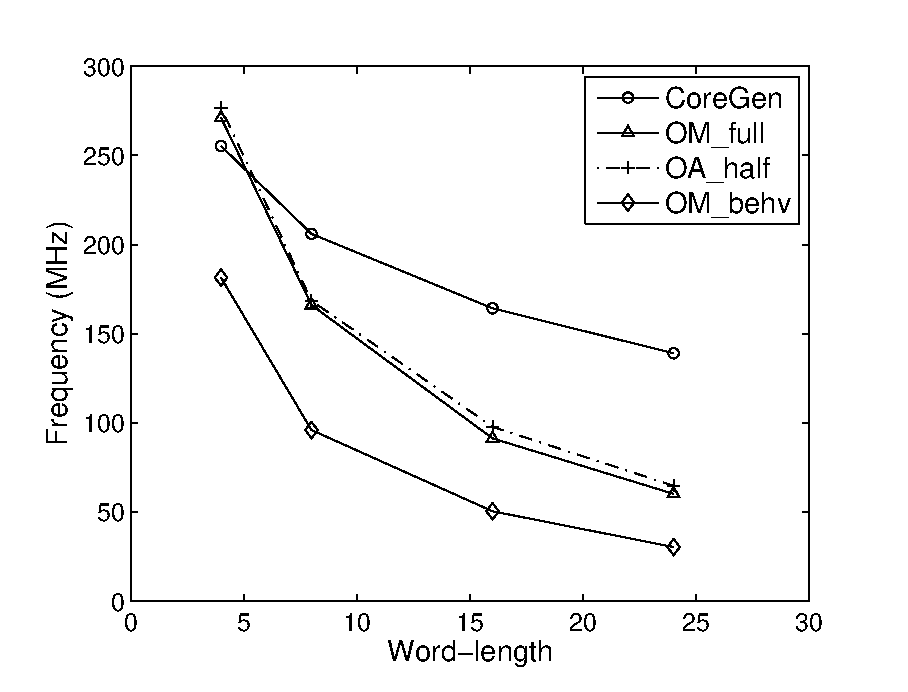
\includegraphics[width=.48\textwidth]{./Figures/Exp/OM_Freq2.eps}
	\caption{Rated frequencies of different types of binary multipliers for a variety of operand word-lengths. The results are obtained from the Xilinx Timing Analyzer in ISE 14.1 after placing and routing.}
	\label{Fig:OM_Freq}

\end{figure}

However, we can take advantage of the ``overclocking friendly'' feature of the online arithmetic, and push the previous tests one step further by operating the circuits beyond their deterministic region while allowing timing violations to happen. We examine the overclocking behavior of all 3 types of multipliers in terms of the mean relative error (\texttt{MRE}), which is given in (\ref{Eq:MRE}), where $E_{error}$ and $E_{out}$ refer to the mean value of error and the mean value of correct output, respectively.

\begin{eqnarray}\label{Eq:MRE}
  MRE=\frac{E_{error}}{E_{out}}\times100\%
  %\vspace{-1ex}
\end{eqnarray}

For instance, Fig.~\ref{Fig:PM_MRE} demonstrates the \texttt{MRE} values of the 8-digit multipliers. The results are from post place and route simulations, and the input stimulus are randomly sampled from a uniform distribution of 8-digit numbers. We see that although the Timing Analyzer predicts slower frequencies for the \texttt{OM}s, they actually operate faster than \texttt{CoreGen} without the occurrence of timing errors. This is in accordance with the results seen in the previous work \cite{SKDAC14_REVIEW}.

\begin{figure}[tbp]
  \centering
  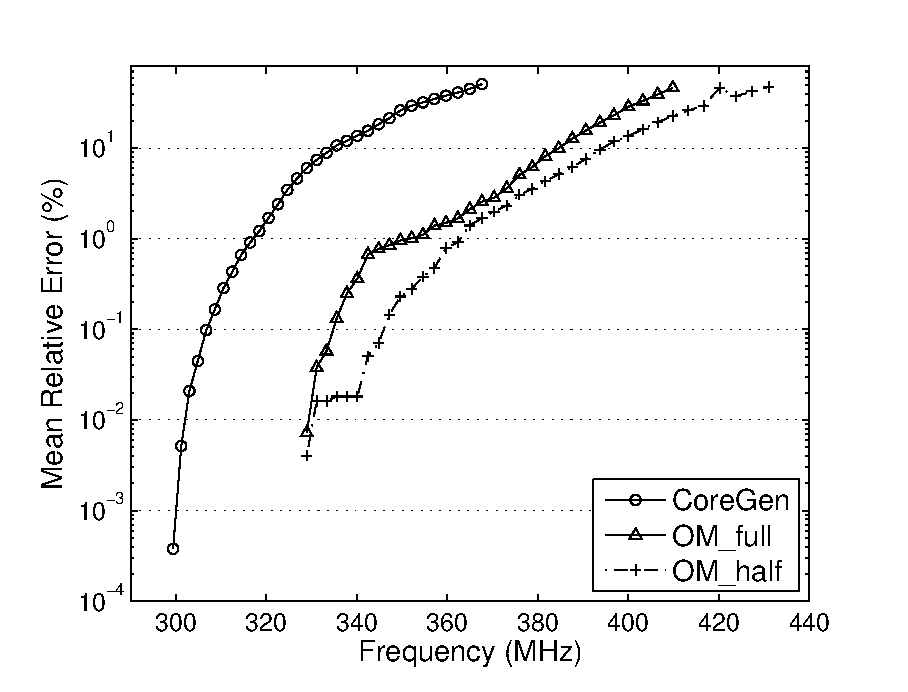
\includegraphics[width=.48\textwidth]{./Figures/Exp/MRE_PM.eps}
 % \vspace{-1ex}
  \caption{Mean relative errors seen at the outputs of different types of 8-digit binary multipliers, when clocked with faster-than-rated frequencies.}
  \label{Fig:PM_MRE}
  %\vspace{-1ex}
\end{figure}


%\section{Results}


% An example of a floating table. Note that, for IEEE style tables, the
% \caption command should come BEFORE the table. Table text will default to
% \footnotesize as IEEE normally uses this smaller font for tables.
% The \label must come after \caption as always.
%
%\begin{table}[!t]
%% increase table row spacing, adjust to taste
%\renewcommand{\arraystretch}{1.3}
% if using array.sty, it might be a good idea to tweak the value of
% \extrarowheight as needed to properly center the text within the cells
%\caption{An Example of a Table}
%\label{table_example}
%\centering
%% Some packages, such as MDW tools, offer better commands for making tables
%% than the plain LaTeX2e tabular which is used here.
%\begin{tabular}{|c||c|}
%\hline
%One & Two\\
%\hline
%Three & Four\\
%\hline
%\end{tabular}
%\end{table}



\section{Conclusion}
In this paper, we initially describe a novel methodology that can efficiently map digit parallel online adders onto FPGAs. The proposed mapping method targets modern FPGAs, which have 6-input LUTs and four LUTs in a slice, and fully utilizes the built-in carry resources. We have demonstrated  that the proposed architecture is both area and performance efficient in comparison to the original design. We then propose an area efficient FPGA implementation of the online multiplier, which is specifically optimized for digit parallel operations. We have shown that this also obtains significant area reduction and frequency speed-ups.

In the future we wish to explore alternative mapping methods for the online multiplier that can effectively use carry resources with long word-lengths to improve  its performance further. We would also like to combine the proposed online primitives into real-world applications.

% conference papers do not normally have an appendix


% use section* for acknowledgement
%\section*{Acknowledgment}




% trigger a \newpage just before the given reference
% number - used to balance the columns on the last page
% adjust value as needed - may need to be readjusted if
% the document is modified later
%\IEEEtriggeratref{8}
% The "triggered" command can be changed if desired:
%\IEEEtriggercmd{\enlargethispage{-5in}}

% references section

\bibliographystyle{./IEEEtran}

% argument is your BibTeX string definitions and bibliography database(s)
%\bibliography{IEEEabrv,../bib/paper}

\bibliography{./IEEEabrv,./Reference}

\end{document}


